%% Template file for all Software/Hardware modules

\subsection{Add-Ons}
The Server provides for the computational needs of the \ac{POW-R} project; 
more hardware shall be added before the utility needs of the project are met.

\subsection{Server Hardware IO}

\subsubsection{\ac{IP} Display}
The \ac{IP} of the Server shall be displayed somewhere on it's casing. 
The user will enter this \ac{IP} into their browser to access the Display.

This will be achieved by connecting an Arduino via \ac{USB} to the Server, and housing it inside the Server's casing. 
The Arduino will be connected to an \ac{LCD} display which will output the network \ac{IP} of the Server. 
Figure \ref{ArduinoLCD} shows the interaction between Server and Arduino.

\begin{figure}
\centering
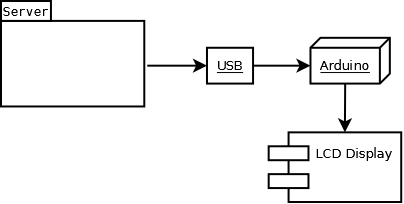
\includegraphics[scale=0.5]{Hardware/images/ArduinoLCD.png}
\caption{\ac{IP} Display Diagram}
\label{ArduinoLCD}
\end{figure}

The \ac{IP} address of the system can be obtained from the operating system, and sent to the Arduino one byte at a time. 
This works well, since the Arduino connects over serial and thusly takes a byte at a time.

\subsubsection{Power Switch}
A standard rocker switch will be added to the case to provide the user with a way to turn the Server on and off. 
The style of the switch will clearly signify "On" or "Off".

\subsubsection{Factory Reset\repeatfootnote{opt}}
This button should intentionally be placed somewhere inconvenient: 
Sunken into the case far enough that you need a skinny rod (such as a paperclip) to push it, and in a spot
that chaotic forces (children, mean people, God's divine will) will not notice it.
	
\subsection{Server Hull}
The Server needs a protective casing for several reasons. 
On the physical level, a durable casing will protect the hardware. 
The casing also serves to render unnecessary ports inaccessible to users. 
Lastly, the casing shall meet client expectations of what a server looks like.

As far as prototyping goes, the casing can be as simple as a folded piece of aluminum
with holes cut in it to fit the \ac{IP} display, the buttons, and any ports that must be
exposed. As an end-game product, the casing would probably be more professional and streamlined.
